% Preamble. Don't worry about it.
\documentclass{article}
\usepackage{setspace,graphicx,fancyhdr}
\usepackage[utf8]{inputenc}
\usepackage[left=1in,top=1in,right=1in,bottom=1in]{geometry} % Document margins
\onehalfspacing

% For custom footers
\pagestyle{fancy}
\fancyhead{}                        % clear all header fields
\renewcommand{\headrulewidth}{0pt}  % no line in header area
\fancyfoot{}                        % clear all footer fields
\fancyfoot[LE,RO]{\thepage}         % for page #s
\fancyfoot[RE,LO]{
\includegraphics{../images/logo/markshark-1x}}

% Setting the depth for Table of Contents
\setcounter{tocdepth}{2}

\begin{document}

% --- TITLE PAGE ---
\title{Donnervögel Consulting \\ MarkShark Grading System \\ Design Document}
\author{\textbf{Phase Lead: Stephen Laboucane} \\ Markus Balaski \\ Ian Pun \\
  Graeme Smith \\ Jordan Toering \\  Colin Woodbury \\ Chazz Young}
\maketitle
\centerline{
\includegraphics{../images/logo/markshark-10x}}
\clearpage
% ------------------

% --- REVISION HISTORY ---
\textbf{Revision History}
\begin{center}
  \begin{tabular}{| c | c | c | l |}
    \hline
    Version & Date & Members & Changes\\
    \hline
    1.0 & 2014 Mar 14 (Fri) & Markus B. & Document created.\\
    & & Graeme S. & \\
    & & Jordan T. & \\
    & & Stephen L. & \\
    & & Ian P. & \\
    & & Colin W. & \\
    & & Chazz Y. & \\
    \hline
  \end{tabular}
\end{center}
\clearpage
% ------------------------

% --- TABLE OF CONTENTS ---
\tableofcontents
\clearpage
% -------------------------

\section{High Level Design}
\subsection{Architecture Diagram}
\centerline{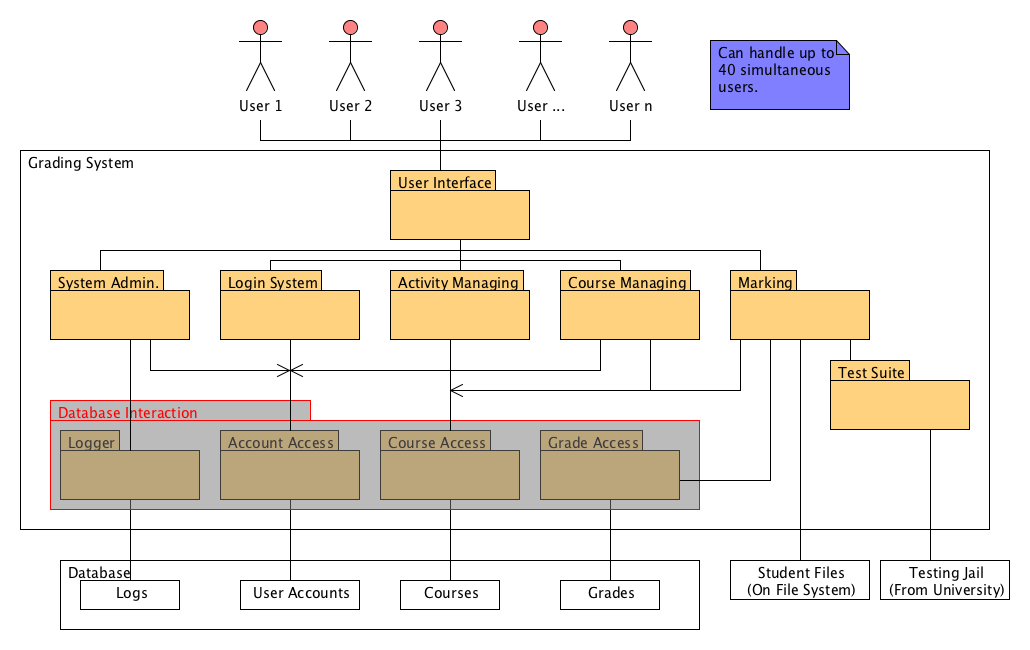
\includegraphics[scale=0.5]{../images/architectureDiagram}}

\subsection{Subsystem Descriptions}
\subsubsection{Main MarkShark Modules}
\begin{itemize}
  \item \textbf{User Interface}: Responsible for the visual portion of the
    application. Accepts user input and handles output.
  \item \textbf{System Administration}: Handles database backups and user
    account creation/modification.
  \item \textbf{Activity Management}: Handles activity creation/modification.
    Contains data related to activity creation forms, etc.
  \item \textbf{Course Management}: Analogous for Courses.
  \item \textbf{Marking}: 
  \item \textbf{Test Suite}:
  \item \textbf{Database Interaction}: Handles all database requests within the
    following smaller modules:
    \begin{itemize}
      \item \textbf{Logger}: Handles the recording of actions performed in the
        system. 
      \item \textbf{Account Access}: Handles requests for user account information
        and conversion between raw database entries into Java classes representing
        the users.
      \item \textbf{Course Access}: Analogous for Course data and Java objects.
      \item \textbf{Grade Access}: Analogous for Grade data and Java objects.
    \end{itemize}
\end{itemize}

\subsection{Refined Use Cases}

\section{Low Level Design}
\subsection{Interaction Diagrams}
\subsection{Class Diagram}

\section{Data Persistence}

\end{document}
